%\chapter{Validation against clinical data}\label{chap2}
\renewcommand{\chaptername}{Chapter} 
\chapter{Psychophysical biomarkers of aprosodia after RH stroke}\label{chap4}

\section{Introduction}
As discussed in Chapter \ref{chap2}, survivors of right-hemisphere stroke may experience deficits in prosody perception that persist from the acute to chronic phase. These impairments can often remain subtle, becoming apparent only in conversations with family members while going undetected during speech therapy sessions when assessed using standard batteries. In this study, our goal was to integrate a reverse correlation experiment into speech therapy sessions. By collecting data from both patients and controls, we aimed to identify cognitive-communication impairments through the application of simple psychophysical models. Validating this prototype would allow us to enhance the specificity of assessments compared to existing tools commonly used by speech therapists.

\section{Materials and methods}
To achieve this, we developed a modified version of the reverse correlation experiment (detailed in Chapter \ref{chap3}) based on the two-alternative forced choice (2AFC) paradigm. Unlike the standard signal detection theory approach, which focuses on target detection, our experiment was designed to probe higher-level processing mechanisms. Specifically, we introduced random Gaussian noise to the base sound for each stimulus \cite{burred_cleese_2019}. This was achieved by recording the utterance of the French word "vraiment" (the equivalent of "really" in English) and generating prosodic variations. The utterance was segmented into six intervals of 71 ms, and the pitch at each breakpoint was independently manipulated using a normal distribution—referred to as stimulus noise. Participants were then asked to judge between two sounds in each trial, identifying which interval contained the manipulated prosodic form of interrogative "vraiment" based on their internal mental representation.

This experiment included repeated trials, following the double-pass paradigm \cite{burgess_visual_1988}, to assess observer consistency by calculating the percentage of agreement in their responses across identical trials. Additionally, it allowed us to measure response bias, identifying whether participants systematically favored one stimulus over the other in repeated passes. By analyzing these responses, we could then simulate the standard deviation of internal noise relative to the scale of external noise, providing insights into the consistency and variability of perceptual decision-making. 

Here, we did not attempt to visualize participants' sensitivity using d-prime since there are no explicitly correct or incorrect responses. Instead, our goal is to estimate their mental representation through correlation mapping. This is achieved by averaging the noisy stimulus from trials where participants provided negative responses and subtracting it from the average noisy stimulus of trials with positive responses. This process results in a weighted sum that reflects their internal representation of the interrogative form of "vraiment".

In our behavioral study, we compare data from right-hemisphere stroke patients (N=22) and age-matched healthy controls (N=21) to establish a baseline for normal prosody perception of the interrogative form of "Vraiment?" This comparison allows us to define a reference threshold for typical performance and identify abnormalities in prosody processing. Additionally, we had the opportunity to incorporate results from various standardized assessment batteries used in speech therapy sessions, serving as pathological gold standards. These included the MEC Comprehension and Repetition tests, Airtac2, LAMA, and MBEA, HADS, which provided valuable clinical benchmarks for validating our findings and assessing the extent of prosodic impairment in patients.

\section{Results}
Both measures extracted from the reverse-correlation procedure effectively distinguished patients from controls. Internal representations of interrogative prosody in the control group exhibited a typical final-rise contour, characterized by a marked pitch increase at the end of the second syllable. Additionally, control participants demonstrated high response consistency across trials, with internal noise values M = 0.7 (SD = 0.37) within the range typically observed for lower-level auditory and visual tasks. In contrast, patients' internal representations had lower amplitude, indicating reduced discriminative power, and displayed greater variability across individuals (M = 2.54, SD = 1.90). Their responses were also associated with significantly higher levels of internal noise. Statistical analyses confirmed significant differences between groups for both representation typicality (p < 0.001) and internal noise (p = 0.001).

Within the patient group, internal noise values—and to a lesser extent, representation typicality—were statistically associated with scores from the current gold standard for assessing prosody perception deficits (MEC), demonstrating good concurrent validity. Higher internal noise values correlated with lower (more severe) scores on the MEC prosody comprehension scale (p = 0.043), while representation typicality showed a positive but non-significant trend (p = 0.15). Notably, neither measure correlated with the MEC prosody repetition score (p = 0.82 and p = 0.365, respectively), despite a significant positive correlation between the two MEC scores. This highlights the symptom specificity of our measures.

A well-known limitation of the MEC instrument is its poor sensitivity, as some patients scoring above the pathological cut-off (9/12) still report communication difficulties. Our measures, however, successfully distinguished this group of MEC-negative (high functoning) patients from controls, both in terms of representation typicality (p = 0.001) and internal noise (p = 0.026).

To further examine the convergent validity and specificity of internal representation and internal noise measures, we explored their associations with other constructs relevant to stroke rehabilitation. As expected, both measures correlated with non-prosody-related difficulties in tone intensity and duration discrimination, as assessed by AIRTAC2 (p = 0.007 and p = 0.037, respectively). However, they were not associated with the ability to detect rare auditory targets among distractors (LAMA, p = 0.25 and p = 0.23) or with musical melody processing, as measured by MBEA (p = 0.46 and p = 0.98).

Regarding musical ability, MBEA was assessed in a subset of patients, the majority of whom were found to have deficits in melody/pitch processing. Among patients classified with melody amusia, 75\% exhibited internal representations that visually deviated from controls, whereas 60\% of non-amusic patients had normal representations. Finally, internal noise—but not representation typicality—was significantly related to anxiety and depression levels, as measured by HADS (p = 0.018 and p = 0.178, respectively).


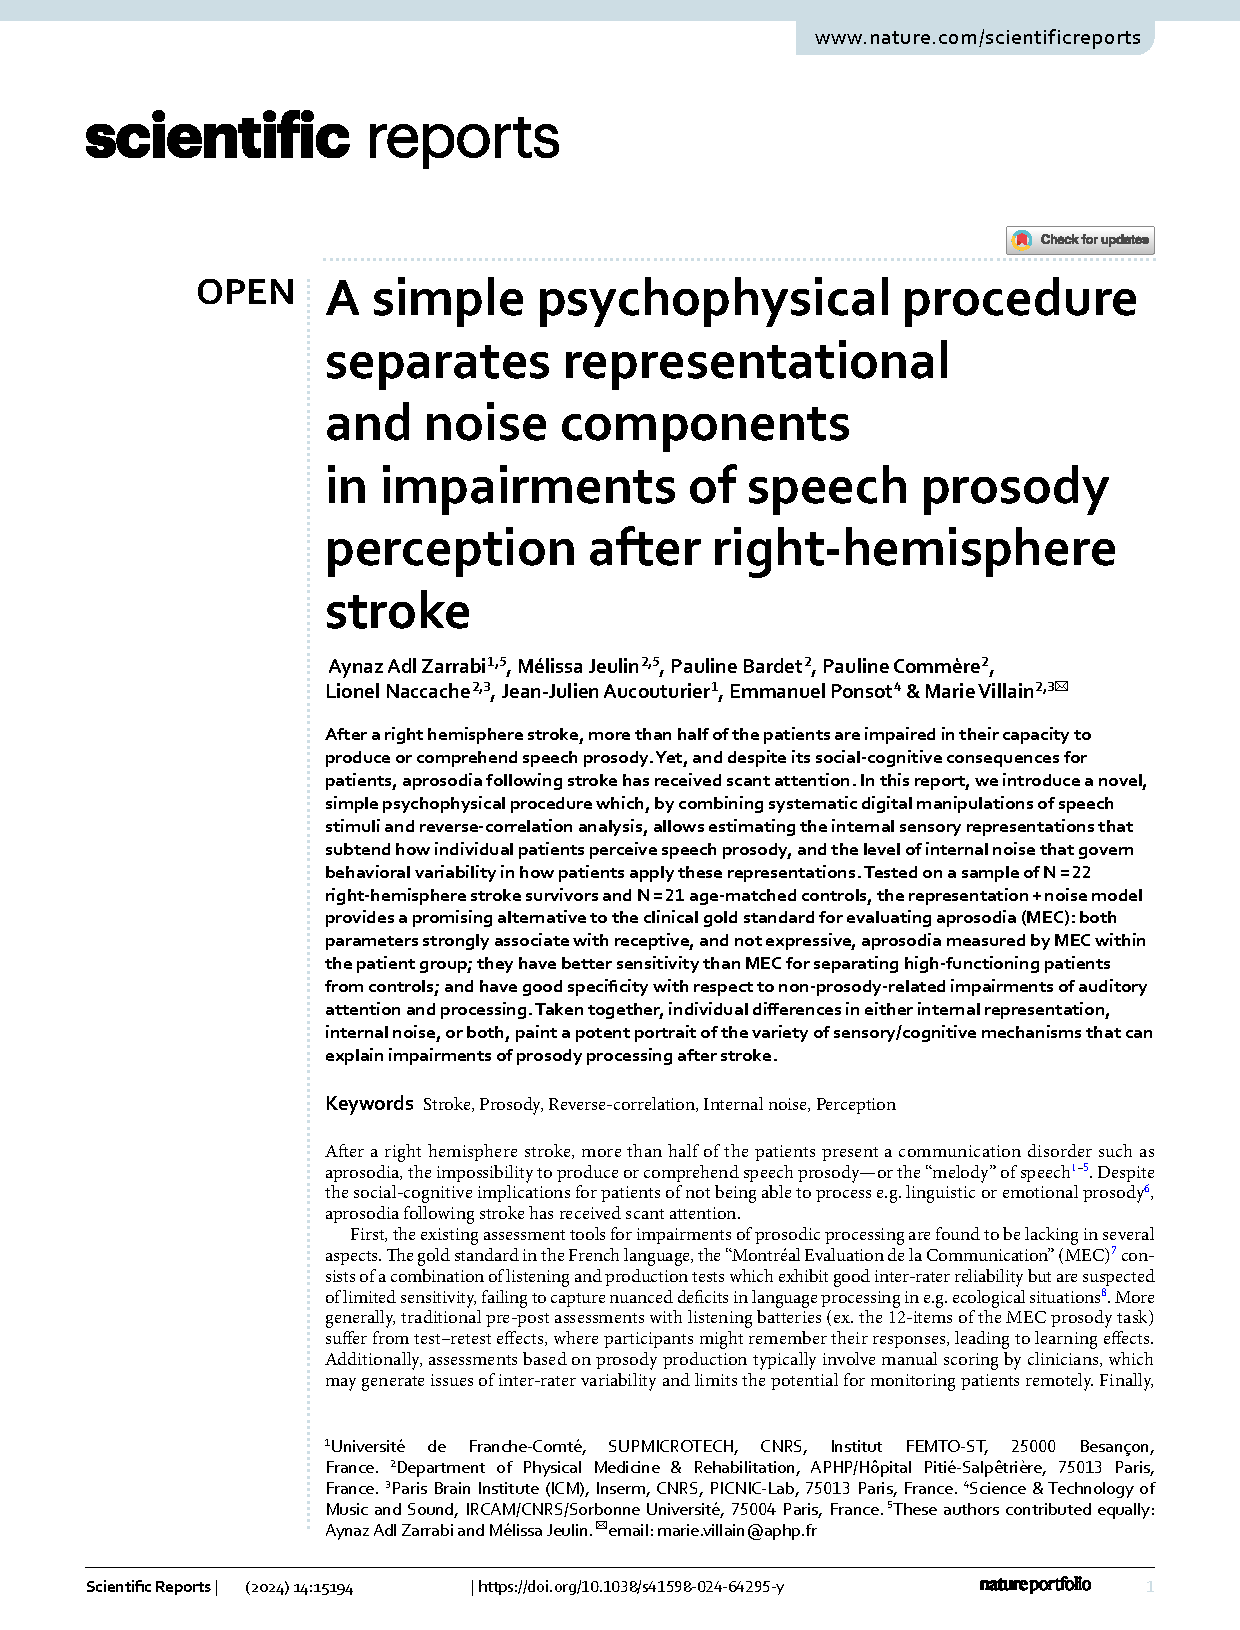
\includepdf[pages=-, scale=0.93, pagecommand={}, offset=0 -0.5cm]{MainLayout/Images/scirep.pdf}

\section {Conclusion: Revcor parameters as potential biomarkers} 
\jj{en quoi cette discussion est différente du chap 5 ? peut-être : dire qu'il y a un potentiel interessant de biomarqueur pour les paramètres revcor: ce qu'on pourrait faire avec, spécificité, etc.}

In this study, we focused on a specific aspect of linguistic prosody: the marking of interrogation through a final pitch rise. Our choice of interrogative prosody serves as a proof of concept rather than a comprehensive test of stroke-related prosodic impairments. The reverse correlation paradigm is highly adaptable and could be applied to various prosodic functions, such as imperative sentences, emotional prosody (e.g., dominance, trustworthiness) \cite{ponsot_cracking_2018}, or other acoustic features like loudness, speech rate \cite{goupil_listeners_2021}, and phonological cues \cite{osses_prosodic_2023}. Its versatility makes it a valuable tool for mechanistically assessing prosodic perception across different contexts. 

Ultimately, representation + noise model offers a framework for understanding prosody impairments after stroke, distinguishing between deficits in internal representations, abnormal internal noise, or a combination of both.

